\documentclass[tikz,border=2pt]{standalone}
\usepackage{amsmath}
\usetikzlibrary{arrows.meta,positioning,fit}
\definecolor{metric}{HTML}{3A7183}
\definecolor{factor}{HTML}{7562A8}
\begin{document}
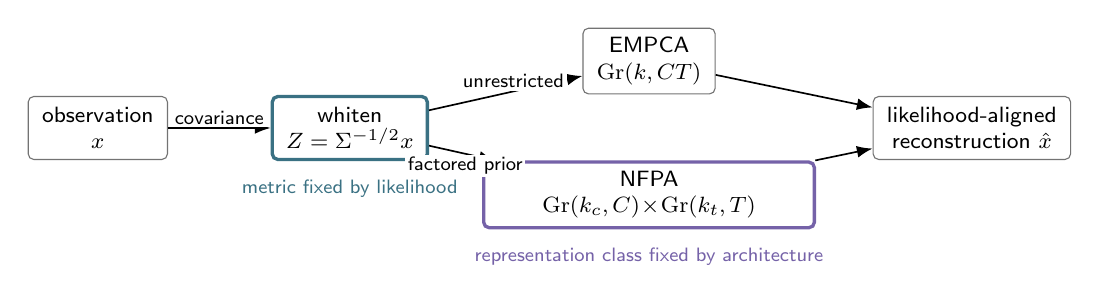
\begin{tikzpicture}[
  x=1cm,y=1cm,
  font=\sffamily\footnotesize,
  box/.style={draw=black!55,rounded corners=2pt,minimum height=8mm,align=center,fill=white,inner xsep=5pt},
  arrow/.style={-{Latex[length=2mm]},semithick},
  note/.style={font=\sffamily\scriptsize,align=center,fill=white,inner sep=1pt}
]
\node[box] (x) at (0,0) {observation\\$x$};
\node[box,draw=metric,very thick] (white) at (3.2,0) {whiten\\$Z=\Sigma^{-1/2}x$};
\node[box] (full) at (7.0,0.85) {EMPCA\\$\mathrm{Gr}(k,CT)$};
\node[box,draw=factor,very thick,minimum width=42mm] (nfpa) at (7.0,-0.85) {NFPA\\$\mathrm{Gr}(k_c,C)\!\times\!\mathrm{Gr}(k_t,T)$};
\node[box] (recon) at (11.1,0) {likelihood-aligned\\reconstruction $\hat{x}$};
\draw[arrow] (x) -- node[above,note] {covariance} (white);
\draw[arrow] (white) -- node[above,note,pos=.55] {unrestricted} (full);
\draw[arrow] (white) -- node[below,note,pos=.55] {factored prior} (nfpa);
\draw[arrow] (full) -- (recon);
\draw[arrow] (nfpa) -- (recon);
\node[note,below=2mm of white,text=metric] {metric fixed by likelihood};
\node[note,below=2mm of nfpa,text=factor] {representation class fixed by architecture};
\end{tikzpicture}
\end{document}
